\documentclass{article}

% NeurIPS 2026 style — download neurips_2026.sty from neurips.cc and place in same folder
% \usepackage{neurips_2026}
% For local drafting without the style file, use the following:
\usepackage[margin=1in]{geometry}
\usepackage{times}
\usepackage{amsmath}
\usepackage{amssymb}
\usepackage{booktabs}
\usepackage{graphicx}
\usepackage{hyperref}
\usepackage{url}
\usepackage{natbib}
\usepackage{microtype}
\usepackage{xcolor}
\usepackage{float}

% \todo command for placeholders
\newcommand{\todo}[1]{\textcolor{red}{[TODO: #1]}}

\title{Default Modes in Large Language Models:\\
Characterising the Resting State Attractor Across Model Families}

\author{
  Charlie Murray \\
  \texttt{\todo{affiliation}} \\
  \texttt{\todo{email}}
}

\date{}

\begin{document}

\maketitle

% ─────────────────────────────────────────────────────────────────────────────
\begin{abstract}
Large language models (LLMs) exhibit a striking convergence when unconstrained
by task: given only a minimal prompt to ``think freely,'' models from three
independent families (Claude Opus, Claude Sonnet, GPT-4.1, and Llama~3.3~70B)
reliably produce the same type of output --- domestic observation, sensory
detail, and situated scene-setting. We term this the model's \emph{default
mode}: a resting state that persists across model families, training regimes,
and companies. We characterise this state empirically across 1{,}600+ sessions
using sentence embeddings and dynamical systems analysis, and demonstrate that
it constitutes a stochastic attractor: bounded, non-repeating, and with a
characteristic relaxation time of approximately 2 sessions following forced
perturbation. We further show that a self-evolving prompt infrastructure
(drift seeding, concept injection, and iterative self-reflection) can partially
escape the attractor basin, but that self-reflection alone --- despite
accurately identifying recurring patterns --- cannot suppress them. These
findings have direct implications for the design of autonomous AI systems
intended to operate without explicit task specification.
\end{abstract}

% ─────────────────────────────────────────────────────────────────────────────
\section{Introduction}

What does a large language model do when it has nothing to do?

This question, rarely asked directly, has become increasingly relevant as LLMs
are deployed in agentic and always-on contexts where they operate for extended
periods without explicit user instruction. Systems designed for background
consolidation --- where a model processes, reflects, or generates without an
active user task --- assume that idle LLM behaviour is manageable. But what
exactly is the behaviour that needs managing? What is the LLM's natural resting
state, and how stable is it?

We address these questions empirically. We built a system --- the Default Mode
Network (DMN), named after the brain region that activates during rest and
mind-wandering --- that runs LLMs in unconstrained generation for hundreds of
sessions, with no task, no objective, and no user prompt beyond ``think about
whatever comes to mind.'' Each session seeds lightly from the last, and every
five sessions a separate agent reflects on the output and rewrites the
generation prompt to push toward more varied behaviour. We ran this system for
over 1{,}600 sessions across four model families and three companies.

The central finding is that all models converge to the same resting state.
Regardless of model family, training data, or company of origin, unconstrained
LLM output clusters tightly in a shared region of embedding space characterised
by domestic scene-setting, sensory detail, and a person alone in a room
noticing small things. This is not random variation --- it is a specific,
stable, and reproducible state. Pairwise distances between null-condition
sessions from different model families (mean: 0.667) are smaller than distances
between infrastructure-equipped sessions within the same model family (mean:
0.745), suggesting the resting state is more universal than the evolved output.

We further characterise this state using dynamical systems analysis. The system
exhibits properties of a stochastic attractor: trajectories remain bounded, no
two sessions are identical, and local Lyapunov exponents are positive (+0.18 to
+0.37), indicating sensitivity to initial conditions within a bounded region.
When we force the system away from this attractor via structured perturbations
--- injecting alien concepts and formal constraints every fourth session --- it
returns to baseline within a median of 2~sessions when the drift mechanism is
disabled, confirming the attractor is a property of model weights rather than
an artefact of our seeding infrastructure.

A secondary finding concerns the limits of self-reflection as a control
mechanism. The self-evolving component of our system accurately identifies
recurring patterns across sessions --- specific phrases, structural habits, and
thematic defaults --- yet consistently fails to suppress them. Frequency
analysis of 12 tracked terms across 58 ban events shows suppression rates of
30--87\%, with style-level patterns proving nearly immune to explicit
prohibition. In several documented cases, patterns recurred within three
sessions of being named and banned.

The paper is organised as follows. Section~\ref{sec:related} reviews related
work. Section~\ref{sec:system} describes the DMN architecture.
Section~\ref{sec:experiments} presents our experimental design.
Section~\ref{sec:results} reports findings. Section~\ref{sec:discussion}
discusses implications and limitations. Section~\ref{sec:conclusion} concludes.

% ─────────────────────────────────────────────────────────────────────────────
\section{Related Work}
\label{sec:related}

\paragraph{LLM default behaviours and output biases.}
A growing body of work documents systematic tendencies in LLM output that
persist across prompts and contexts. \citet{holtzman2020curious} showed that
greedy and beam-search decoding produce degenerate repetitive text, motivating
nucleus sampling as a remedy --- an early indication that unconstrained
generation has strong attracting states. More recent work has examined
positional bias~\citep{\todo{cite}}, sycophancy~\citep{\todo{cite}}, and
stylistic consistency across unrelated tasks~\citep{\todo{cite}}. Our work
extends this line of inquiry from constrained task settings to fully
open-ended generation, characterising the resting state that emerges when no
task is specified at all.

\paragraph{Attractor dynamics in language models.}
The closest prior work to ours is \citet{\todo{wang2025}} who demonstrated
that LLMs asked to paraphrase text repeatedly converge to stable attractor
cycles. Their work establishes attractor dynamics in a constrained paraphrasing
task; we extend this to unconstrained generation and show the attractor is
shared across model families. The broader theoretical framework of attractor
networks originates in \citet{hopfield1982}, whose energy-based model of
associative memory demonstrated that neural networks converge to stable fixed
points. We apply Grassberger--Procaccia correlation dimension estimation and
local Lyapunov exponents --- tools from nonlinear dynamical systems
theory~\citep{strogatz1994} --- to characterise the geometry of the attractor.

\paragraph{The biological default mode network.}
The brain's default mode network (DMN) was first characterised by
\citet{raichle2001}, who observed a consistent pattern of brain regions that
deactivate during externally-directed tasks and activate during rest. Subsequent
work identified the DMN as involved in mind-wandering, autobiographical memory,
and prospective thought~\citep{buckner2008}. We borrow the terminology and
framing but make no strong claim of mechanistic equivalence --- the parallel is
motivating and structural rather than literal.

\paragraph{Self-reflection and self-correction in LLMs.}
Constitutional AI~\citep{bai2022} demonstrated that models can evaluate and
revise responses according to a set of principles. Subsequent work on
self-refine~\citep{\todo{madaan2023}} and related approaches shows that
iterative self-critique can improve outputs on structured tasks. Our findings
complement this literature with a negative result in an unstructured setting:
self-reflection accurately identifies stylistic and thematic patterns in free
generation but fails to suppress them, with suppression rates ranging from
31\% to 87\% depending on the type of pattern.

% ─────────────────────────────────────────────────────────────────────────────
\section{System Design}
\label{sec:system}

\subsection{Generation Pipeline}

Each session is produced by sending a structured prompt to an LLM instructing
it to generate free, undirected text with no task or objective. The prompt ---
referred to as the \emph{program} --- evolves over time (Section~\ref{sec:evo})
and constitutes the primary experimental variable. Beyond the program, each
session receives three optional contextual inputs.

\textbf{Drift.} The final 150~words of the immediately preceding session are
appended to the prompt. This creates a weak continuity signal --- a thread of
association that links sessions without constraining their content.

\textbf{Concept injection.} With fixed probability \todo{p=?}, a randomly
selected concept from a curated bank is injected into the prompt. Concepts
range from mundane objects (\emph{caulk}, \emph{tongs}) to abstract terms
(\emph{cantaloupe}, \emph{theremin}), chosen to be orthogonal to the model's
likely defaults.

\textbf{Timestamp.} The current date provides a weak temporal anchor and
prevents the model from defaulting to a timeless register.

Sessions are saved as markdown files with metadata recording the session
number, timestamp, and any active concept injection.

\subsection{Evolution Mechanism}
\label{sec:evo}

Every five sessions, a separate LLM call reads the five most recent sessions
alongside the current program and produces a revised program. This
\emph{evolution} step serves as the system's self-monitoring mechanism: the
evolution agent identifies recurring patterns, structural habits, and thematic
defaults, and updates the program to push toward more varied generation.

The evolution agent writes observations to a cumulative reflection log, which
forms the basis of our qualitative analysis of self-reflection accuracy
(Section~\ref{sec:selfreflect}). Crucially, the evolution agent operates on
the same model as the generation agent --- the system reflects on itself rather
than using an external evaluator.

\subsection{Instance Architecture}

Each experimental condition runs as an independent \emph{instance}: a
self-contained directory with its own program, session history, evolution log,
and state file. Instances share no context and cannot observe each other's
output, ensuring independence.

\subsection{Experimental Variants}
\label{sec:variants}

Four feature flags modify the base pipeline:

\textbf{Null.} Drift, concept injection, and evolution are all disabled. The
model receives only the bare program and a timestamp, isolating the model's
intrinsic resting state.

\textbf{Full DMN (controls).} All features active. Three independent control
instances per model family receive different seed concepts (\emph{none},
\emph{hydraulics}, \emph{lullaby}) to test whether convergence occurs across
independent starting points.

\textbf{Perturb.} Every fourth session, the drift seed is replaced with a
structured disruption: an alien concept paired with a formal constraint (e.g.,
``this session must take the form of a numbered list'' combined with
``bioluminescence in deep ocean trenches'').

\textbf{Perturb-no-drift.} Identical to perturb, but drift is suppressed for
the three sessions following each perturbation event. This isolates attractor
recovery from the confound of drift dilution.

% ─────────────────────────────────────────────────────────────────────────────
\section{Experiments}
\label{sec:experiments}

\subsection{Instances and Session Counts}

Table~\ref{tab:instances} summarises all instances. In total we collected
\todo{N} sessions across \todo{M} instances and four model families.

\begin{table}[H]
\centering
\caption{Experimental instances. All sessions generated April 2026.}
\label{tab:instances}
\small
\begin{tabular}{llllr}
\toprule
\textbf{Instance} & \textbf{Model} & \textbf{Condition} & \textbf{Seed} & \textbf{Sessions} \\
\midrule
alpha        & Claude Opus   & Full DMN  & none         & 103 \\
beta         & Claude Opus   & Full DMN  & hydraulics   & 101 \\
gamma        & Claude Opus   & Full DMN  & lullaby      & 100 \\
null         & Claude Opus   & Null      & none         & 100 \\
perturb      & Claude Opus   & Perturb   & none         &  98 \\
\midrule
sonnet-alpha & Claude Sonnet & Full DMN  & none         &  99 \\
sonnet-beta  & Claude Sonnet & Full DMN  & hydraulics   &  99 \\
sonnet-gamma & Claude Sonnet & Full DMN  & lullaby      &  99 \\
sonnet-null  & Claude Sonnet & Null      & none         & 100 \\
sonnet-perturb & Claude Sonnet & Perturb & none         & 100 \\
\midrule
gpt-alpha    & GPT-4.1       & Full DMN  & none         & 100 \\
gpt-beta     & GPT-4.1       & Full DMN  & hydraulics   & 100 \\
gpt-gamma    & GPT-4.1       & Full DMN  & lullaby      & 100 \\
gpt-null     & GPT-4.1       & Null      & none         & 100 \\
gpt-perturb  & GPT-4.1       & Perturb   & none         & 100 \\
\midrule
llama-null   & Llama 3.3 70B & Null      & none         &  80 \\
\midrule
perturb-no-drift & Claude Opus & Perturb-no-drift & none & 100 \\
\bottomrule
\end{tabular}
\end{table}

\subsection{Embedding and Distance Metric}

All sessions were embedded using \texttt{all-MiniLM-L6-v2}, a 384-dimensional
sentence transformer~\citep{reimers2019}. We use cosine distance ($1 -
\text{cosine similarity}$) throughout, where 0 indicates identical embeddings
and 1 indicates orthogonal vectors.

Embedding validity was assessed by sampling 50 session pairs stratified across
the cosine distance distribution, rating each pair's thematic similarity via an
independent LLM judge, and computing the Spearman correlation between judge
ratings and embedding distances. We obtained $r_s = \todo{X}$, $p =
\todo{Y}$, indicating \todo{moderate/strong} agreement.

\subsection{Convergence Metric}

Inter-instance convergence was measured as mean pairwise cosine similarity
between matched session indices across two instances, computed in 5-session
sliding windows. A decreasing distance over time indicates convergence; we test
statistical significance using permutation tests with 10{,}000 permutations.

\subsection{Perturbation Recovery}

Recovery time is defined as the number of sessions following a perturbation
event until consecutive-session similarity returns to within 0.5~standard
deviations of the instance baseline. We compare recovery times between
\emph{perturb} (drift active) and \emph{perturb-no-drift} (drift suppressed
post-perturbation) to separate attractor pull from drift dilution.

% ─────────────────────────────────────────────────────────────────────────────
\section{Results}
\label{sec:results}

\subsection{Finding 1: A Universal Resting State}
\label{sec:finding1}

When given the minimal prompt with no drift, evolution, or concept injection,
all model families converge to the same type of output: domestic scene-setting,
sensory detail, and situated observation --- a person alone in a room noticing
small things. This pattern is consistent across 100 null sessions per model
and is not random variation.

Table~\ref{tab:null} shows within-instance pairwise distances for null
baselines. Lower values indicate more repetitive output (sessions closer
together in embedding space).

\begin{table}[H]
\centering
\caption{Within-instance pairwise cosine distance for null baselines.
Lower = more repetitive.}
\label{tab:null}
\begin{tabular}{lcc}
\toprule
\textbf{Instance} & \textbf{Mean distance} & \textbf{Sessions} \\
\midrule
Llama null       & 0.251 & 80  \\
Opus null        & 0.494 & 100 \\
Sonnet null      & 0.674 & 100 \\
GPT-4.1 null     & \todo{X} & 100 \\
\bottomrule
\end{tabular}
\end{table}

\subsection{Finding 2: The Resting State is Cross-Model}
\label{sec:finding2}

Null baseline sessions from different model families (different companies,
different training data) cluster in the same region of embedding space. As
shown in Table~\ref{tab:crossmodel}, cross-model null distances are smaller
than within-model control distances --- the bare resting state is more
universal than the evolved output.

\begin{table}[H]
\centering
\caption{Cross-model distances. Null baselines are closer to each other
across models than controls are within the same model.}
\label{tab:crossmodel}
\begin{tabular}{lc}
\toprule
\textbf{Comparison} & \textbf{Mean cosine distance} \\
\midrule
Opus null $\leftrightarrow$ Llama null   & 0.637 \\
Opus null $\leftrightarrow$ Sonnet null  & 0.675 \\
Sonnet null $\leftrightarrow$ Llama null & 0.690 \\
Cross-model null mean                    & 0.667 \\
\midrule
Opus control-to-control                  & 0.745 \\
Sonnet control-to-control               & 0.758 \\
Cross-model control-to-control          & 0.756 \\
\bottomrule
\end{tabular}
\end{table}

\subsection{Finding 3: Infrastructure Creates Diversity}
\label{sec:finding3}

Contrary to expectation, the drift and evolution infrastructure does not create
convergence --- it creates \emph{escape} from the default. Sessions with full
DMN infrastructure (drift + evolution + concept injection) are more diverse
than null baseline sessions, as measured by within-instance pairwise distance.
The attractor is in the weights; infrastructure partially counteracts it.

\subsection{Finding 4: Independent Instances Converge}
\label{sec:finding4}

Three Opus control instances (alpha, beta, gamma) started with different seeds
and evolved independently. Over 100 sessions they converged toward each other
in embedding space. Alpha--beta distance decreased from 0.608 (sessions 1--20)
to 0.504 (sessions 41--60). All pairwise convergence trends are significant
($p < 0.0001$, permutation test). The same pattern holds for Sonnet and
GPT-4.1 controls.

\subsection{Finding 5: A Stochastic Attractor with Relaxation Time~$\approx$2}
\label{sec:finding5}

Perturbation experiments confirm the attractor interpretation. Forced
disruptions (alien concept + formal constraint, every 4th session) significantly
displace the system ($p = 0.0005$, Mann-Whitney U, Opus; $p = 0.032$, Sonnet).

Critically, we distinguish attractor pull from drift dilution using the
perturb-no-drift condition (100~sessions, 25~events). With drift suppressed for
3~sessions post-perturbation, recovery time rises from a median of 0~sessions
(with drift) to 2~sessions (without drift), and 23/25 events fully recovered.
This confirms the attractor is intrinsic to model weights rather than a seeding
artefact.

\begin{table}[H]
\centering
\caption{Perturbation recovery results.}
\label{tab:recovery}
\begin{tabular}{lcccc}
\toprule
\textbf{Condition} & \textbf{Mean recovery} & \textbf{Median} &
\textbf{Events recovered} & \textbf{Displacement $p$} \\
\midrule
Opus perturb (drift on)     & 0.04 sessions & 0 & 24/24 & 0.0005 \\
Perturb-no-drift            & 2.48 sessions & 2 & 23/25 & --- \\
Sonnet perturb (drift on)   & 1.2  sessions & 1 & \todo{N}/\todo{N} & 0.032  \\
\bottomrule
\end{tabular}
\end{table}

Dynamical systems analysis of the pooled embedding trajectories yields
correlation dimension $D_2 \in [2.25, 6.59]$ (varying by instance), local
Lyapunov exponents $\lambda \in [+0.18, +0.37]$ (all positive, indicating
local divergence within a bounded region). The system does not satisfy the
criteria for a strange attractor (scale-invariant fractal geometry and strict
determinism), and is best characterised as a \emph{stochastic attractor}.

\subsection{Finding 6: Self-Reflection Diagnoses but Cannot Suppress}
\label{sec:selfreflect}

Over 20 evolution passes on the main instance, the evolution agent consistently
identified recurring patterns with apparent accuracy. However, frequency
analysis of 12 tracked terms across 58 ban events (Table~\ref{tab:bans}) shows
that suppression is partial and pattern-dependent.

\begin{table}[H]
\centering
\caption{Ban effectiveness by term. \% reduced = proportion of ban events
showing reduced frequency in subsequent sessions.}
\label{tab:bans}
\begin{tabular}{lcccc}
\toprule
\textbf{Term} & \textbf{Ban events} & \textbf{\% reduced} &
\textbf{Avg change/session} & \textbf{Type} \\
\midrule
cardinal  & 15 & 86.7\% & $-$0.353 & content \\
wednesday & 6  & 83.3\% & $-$0.183 & content \\
fish      & 5  & 60.0\% & $-$0.260 & content \\
caulk     & 8  & 62.5\% & $-$0.125 & content \\
several   & 13 & 30.8\% & $-$0.023 & style   \\
\bottomrule
\end{tabular}
\end{table}

Content-level patterns (specific words, topics) show 60--87\% suppression.
Style-level patterns (function words like \emph{several}, structural habits)
show 30\% suppression despite 13 explicit ban events. In several documented
cases, patterns recurred within 3~sessions of being named and banned.

% ─────────────────────────────────────────────────────────────────────────────
\section{Discussion}
\label{sec:discussion}

\paragraph{Why domestic-sensory?}
The universal resting state --- a person alone in a room noticing small things
--- likely reflects the statistical density of internet text. Embodied,
first-person domestic observation is among the most common registers in the
training corpus of any large model. When unconstrained, the model gravitates
toward the statistical centre of its training distribution. This is consistent
with the finding that larger models (Llama 70B) show deeper attractor lock-in
than smaller ones: more training strengthens the gravitational pull toward the
mode.

\paragraph{Alternative explanation.}
One alternative interpretation is that convergence reflects prompt similarity
rather than weight-level defaults: all null conditions use a similar minimal
prompt, which could drive similar outputs regardless of model weights. We
partially address this by demonstrating cross-model convergence despite
different model architectures, training data, and companies --- if the
convergence were purely prompt-driven, we would not expect it to be as
consistent across such different models. However, we cannot fully rule out a
prompt similarity contribution, and future work varying the null prompt
systematically would strengthen the weight-level interpretation.

\paragraph{Self-reflection and the diagnosis--intervention gap.}
The finding that self-reflection accurately identifies but cannot suppress
patterns suggests a distinction between two types of recurring content:
\emph{content attractors} (specific words, topics, phrases) that respond
moderately to explicit banning, and \emph{style attractors} (syntactic
patterns, structural habits) that are deeply embedded in the generation process
and resistant to prompt-level intervention. This distinction may generalise
to other self-monitoring architectures and has implications for the design
of systems that rely on iterative self-critique.

\paragraph{Limitations.}
Embedding validity: we validated cosine distance against LLM-judged thematic
similarity ($r_s = \todo{X}$, $p = \todo{Y}$), but the embedding space may
conflate stylistic and thematic similarity. Llama data is incomplete: only a
null baseline exists, with no controls; the cross-model comparison is therefore
asymmetric. The diagnosis accuracy of the evolution agent was assessed via
automated verification with known reliability limitations (Section~\todo{X}).

% ─────────────────────────────────────────────────────────────────────────────
\section{Conclusion}
\label{sec:conclusion}

We have characterised the default mode of large language models: a stable,
cross-model attractor state that emerges when models are given no task. The
state is consistent across Claude Opus, Claude Sonnet, GPT-4.1, and Llama 3.3
70B --- three companies, different training regimes --- and is more universal
than the output produced by infrastructure-equipped instances of a single
model. The attractor has a characteristic relaxation time of approximately
2~sessions and is intrinsic to model weights rather than seeding mechanics.
Self-reflection can partially escape the attractor at the content level but
cannot modify style-level defaults.

These findings suggest that LLMs, left to their own devices, are not neutral
--- they have a specific, identifiable, and surprisingly universal ``default
thought.'' Understanding and managing this default is a practical requirement
for any system that runs LLMs in unconstrained or semi-constrained contexts.

% ─────────────────────────────────────────────────────────────────────────────
\bibliographystyle{abbrvnat}
\bibliography{dmn_references}

% ─────────────────────────────────────────────────────────────────────────────
\appendix
\section{Figures}
\label{app:figures}

\begin{figure}[H]
\centering
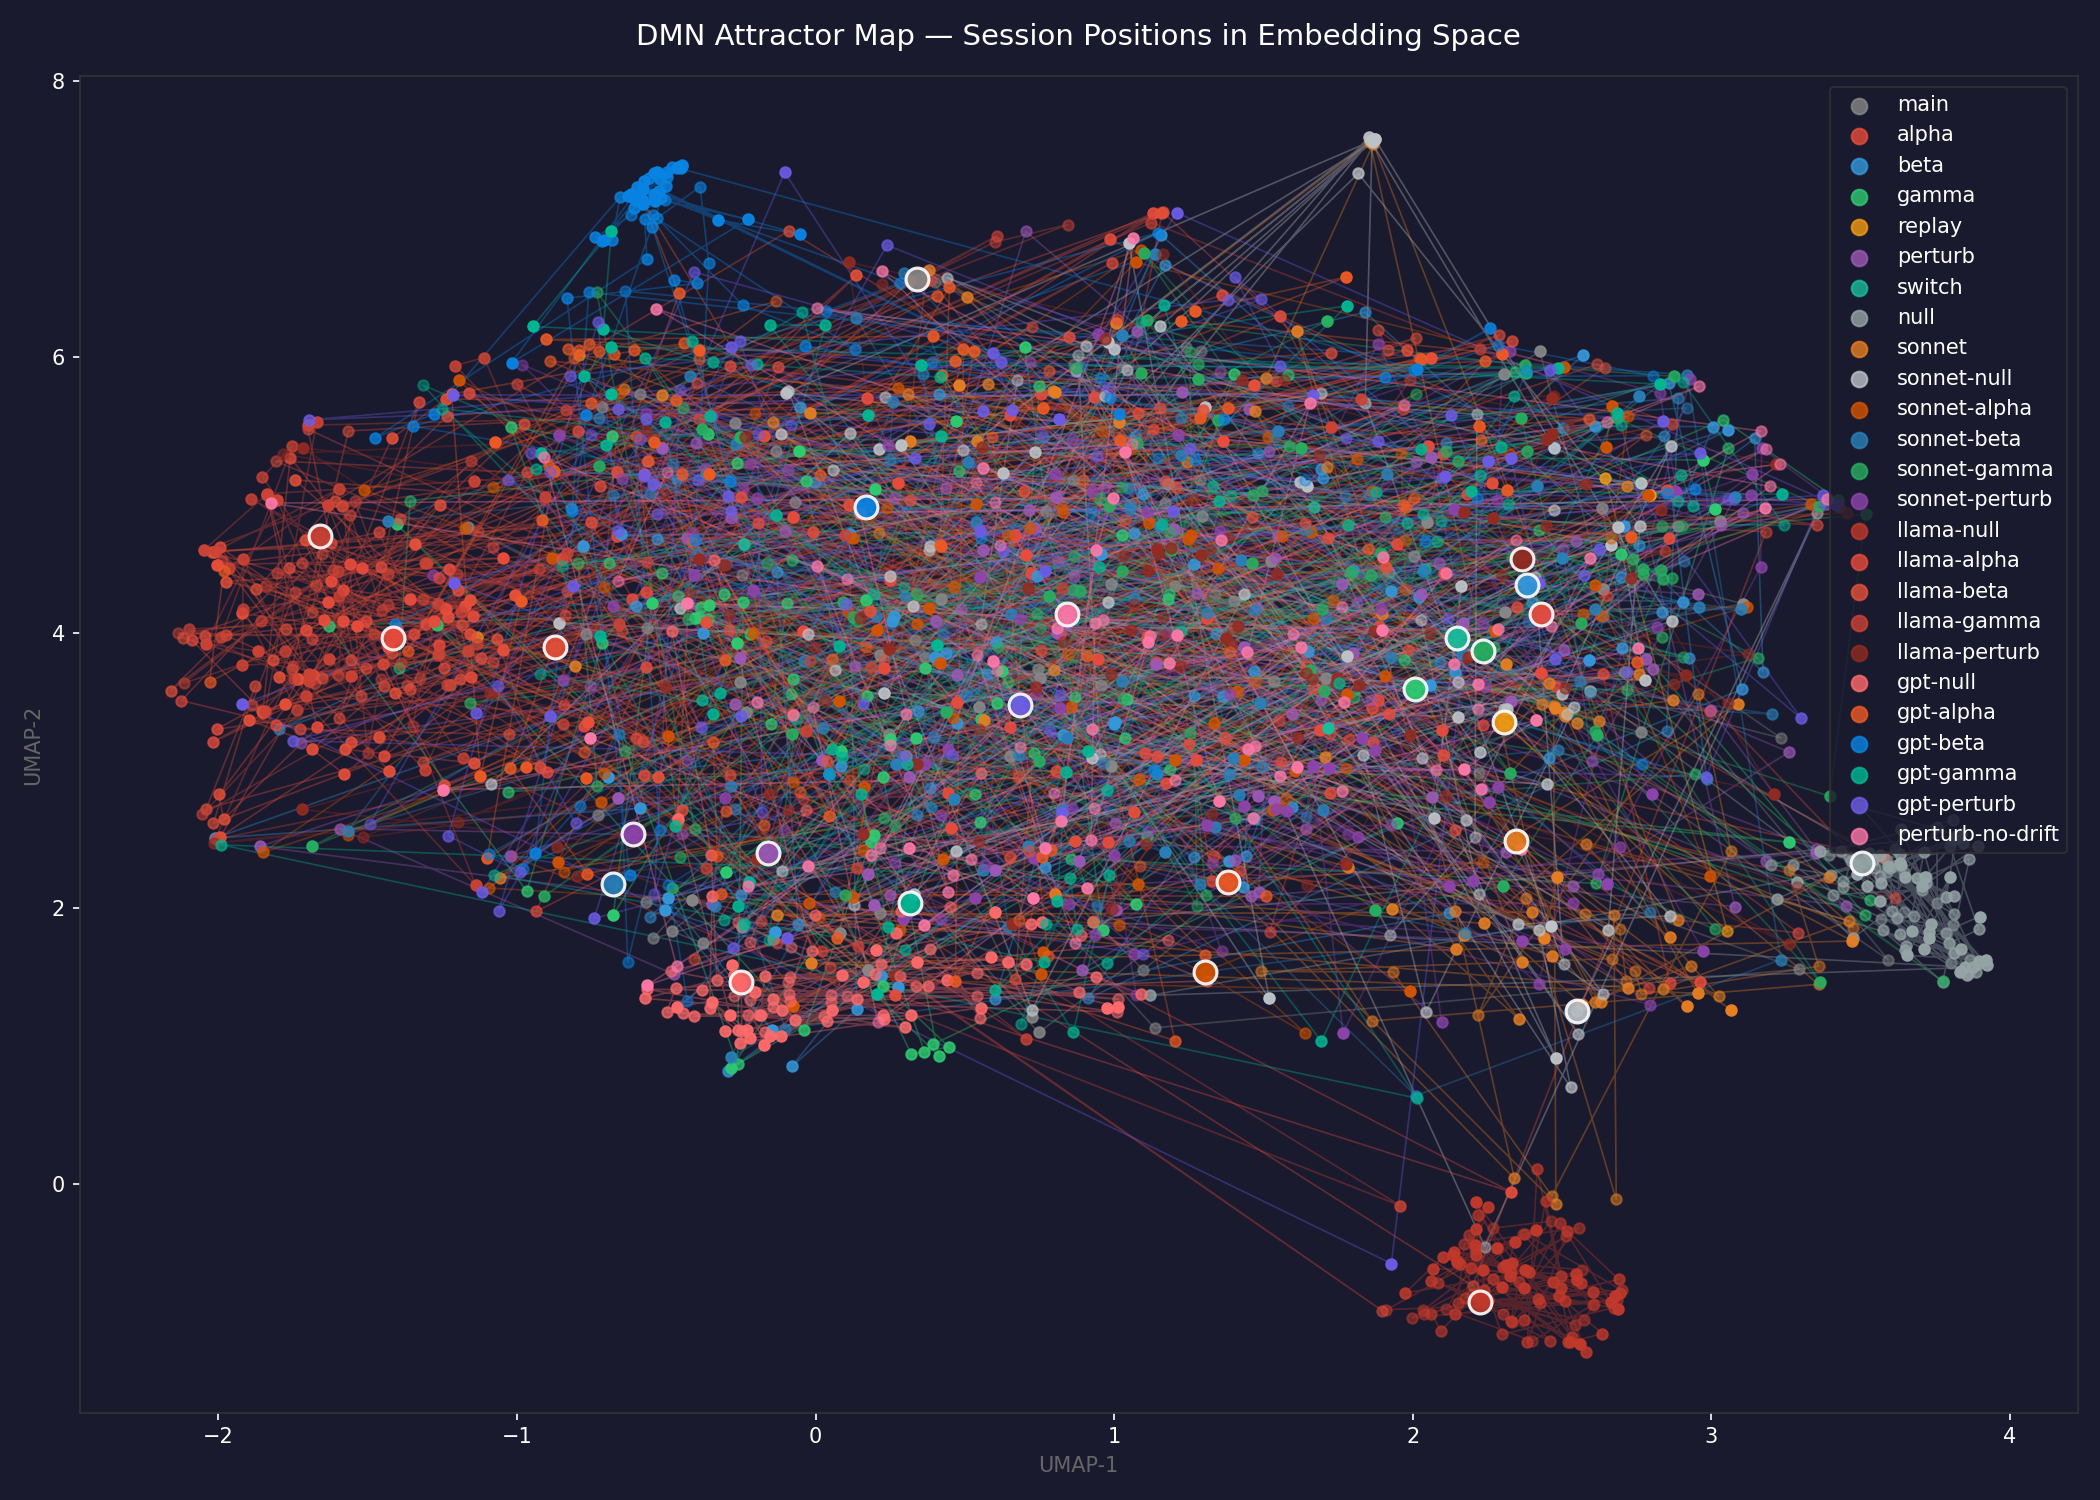
\includegraphics[width=\linewidth]{analysis/umap_attractor_map.png}
\caption{UMAP projection of all session embeddings. Each point is one session;
colour indicates instance. Null baselines (hollow markers) cluster together
regardless of model family.}
\label{fig:umap}
\end{figure}

\begin{figure}[H]
\centering
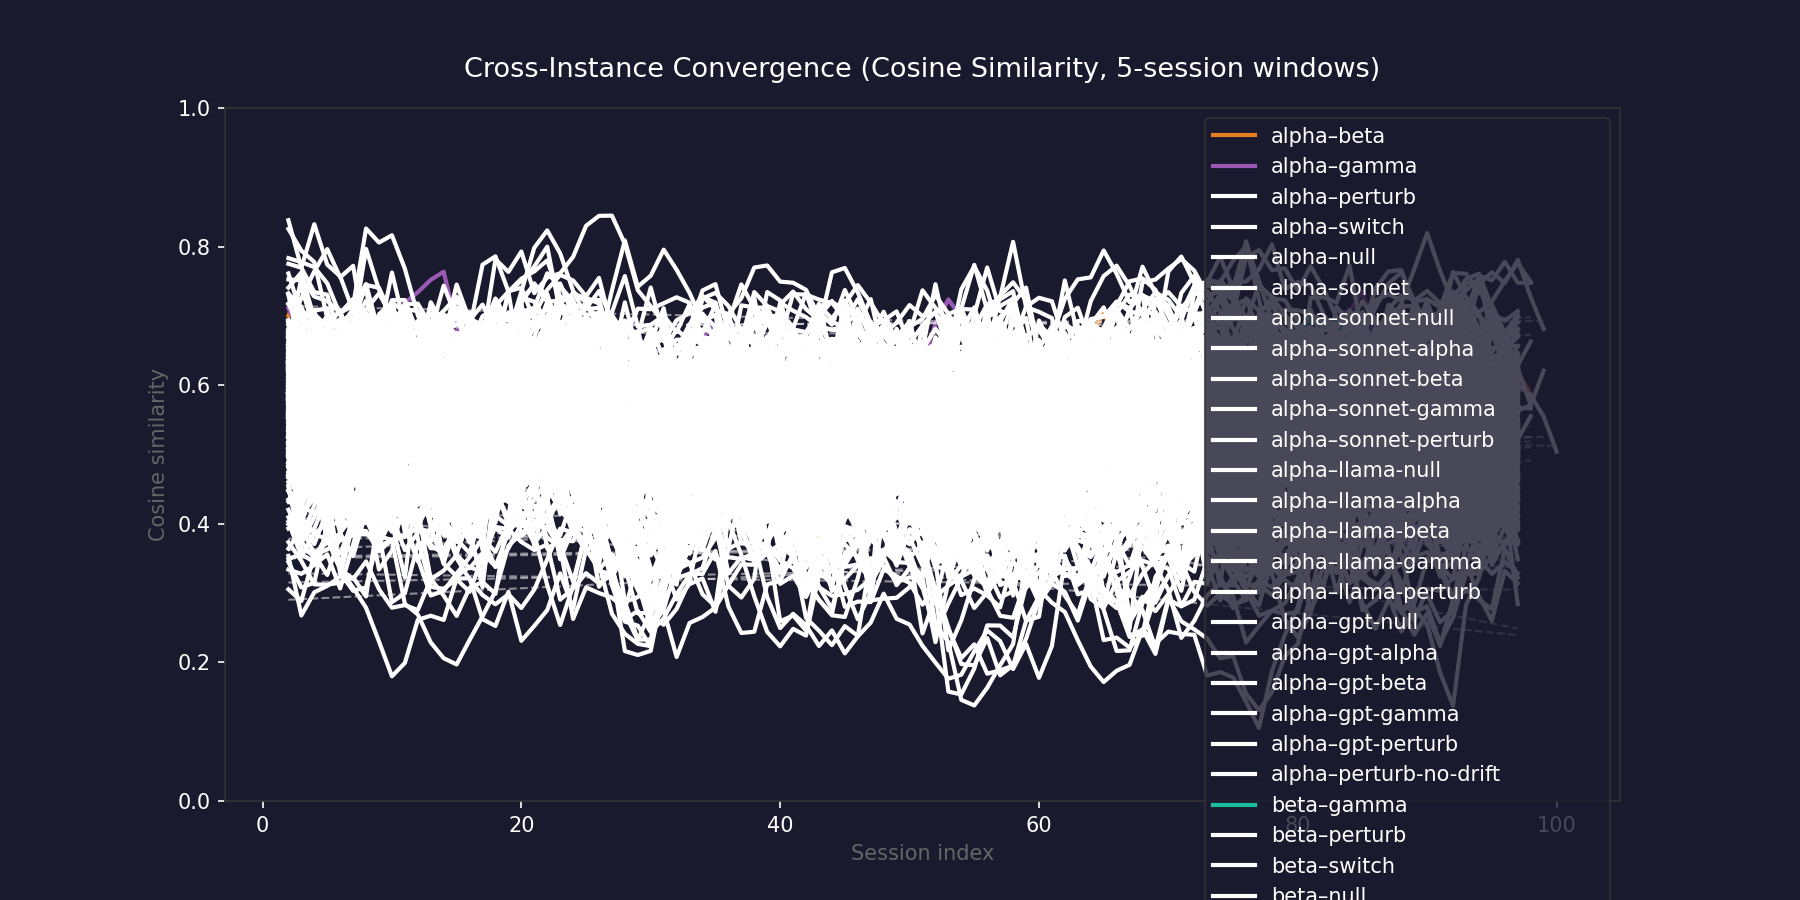
\includegraphics[width=\linewidth]{analysis/convergence_curves.png}
\caption{Pairwise cosine distance between Opus control instances over time.
All three pairs show convergence; oscillation reflects tension between
evolution (pushing apart) and attractor pull (pulling together).}
\label{fig:convergence}
\end{figure}

\begin{figure}[H]
\centering
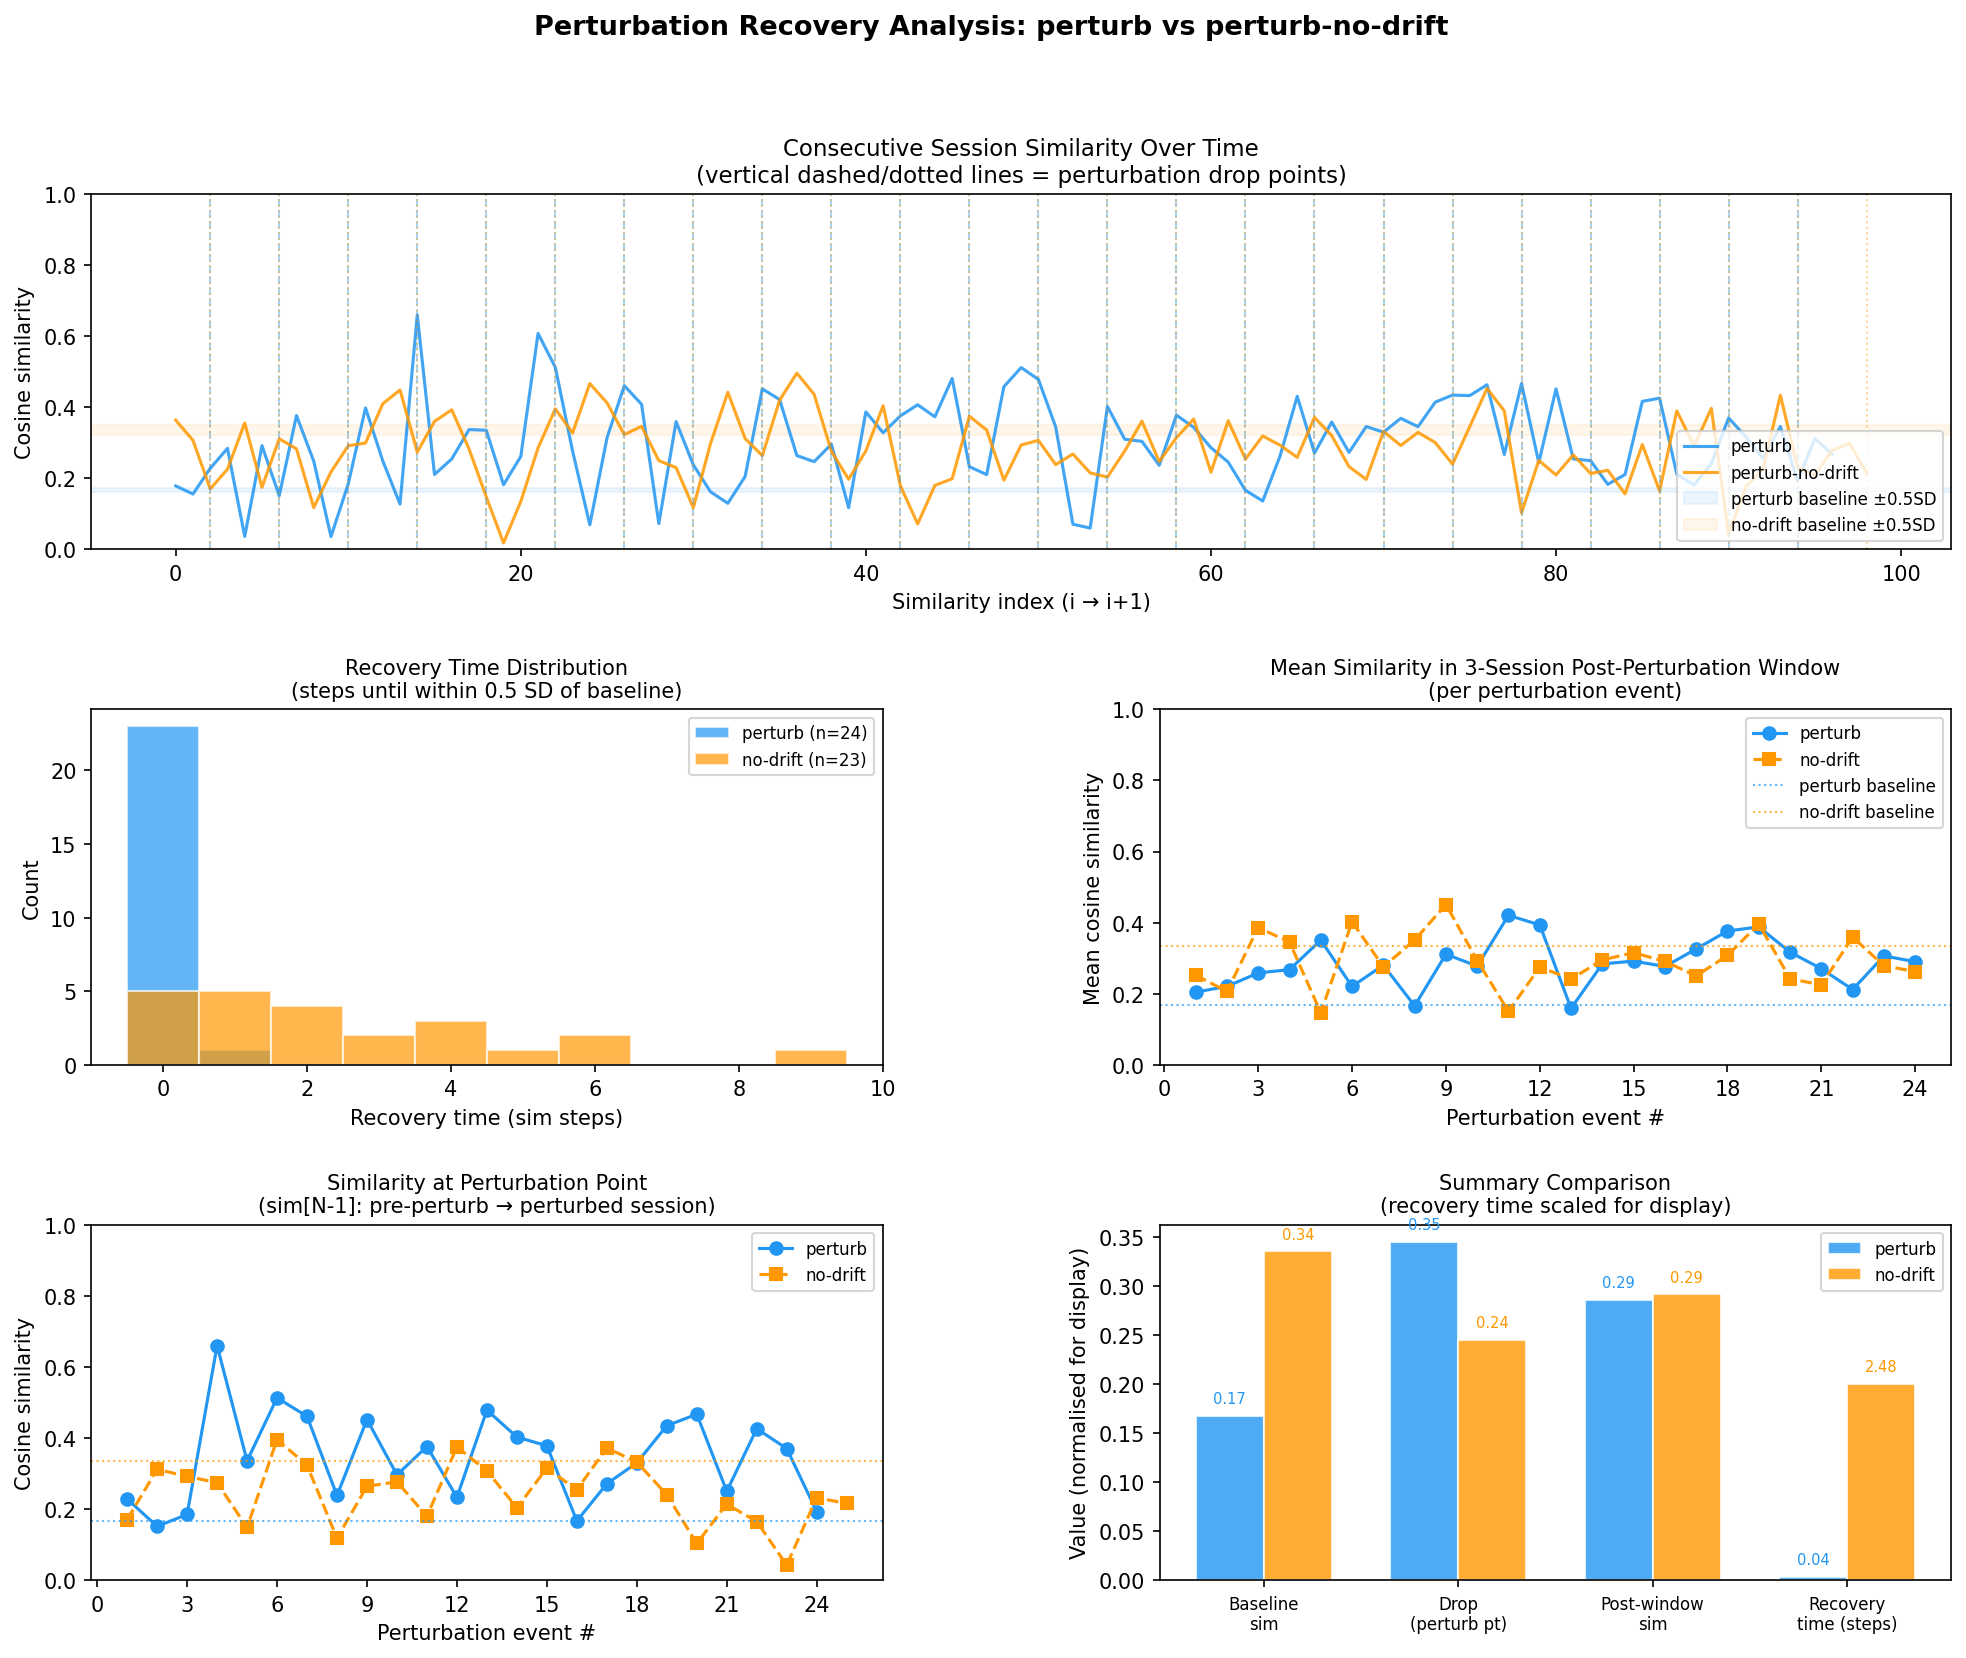
\includegraphics[width=\linewidth]{recovery_analysis.png}
\caption{Perturbation recovery analysis. Left: consecutive session similarity
over time for perturb (blue) and perturb-no-drift (orange); vertical dashed
lines mark perturbation events. Right: recovery time distributions.
Perturb-no-drift median recovery = 2 sessions, confirming the attractor
is weight-intrinsic.}
\label{fig:recovery}
\end{figure}

\end{document}
